\chapter{Use, Scope and Limitations of RFID Technology}
\label{Kap1}

The following chapter will discuss the reasons why to choose the RFID technology. In the beginning, in the 'Motivation' section there will be described some state of the art applications. After that, the section 'Aim and Scope' will introduce the limits of the RFID technology and of its applications which should be considered during the deployment. In the end, there will be outlined the \ac{SWOT} method to analyze the benefits and threats of an RFID application.

\section{Motivation}

Concerning the organization and management of medical devices or patients in a hospital, there exist many problems. In the following, some solutions to these problems, as described by Ajami and Rajabzadeh \cite{ncbi}, will be depicted.

\subsection{Decision Making}

First of all, when it comes to decision making, e.g. about the correct treatment of a severe illness, many physicians are stumped for an answer or their opinions are divided. To enable a rapid diagnosis and to improve the patient's health status, 'smart healthcare' \cite{henrici} would help a lot. 'Smart healthcare' includes RFID tags which are equipped with sensors to ensure the effectiveness of a medical treatment. This accelerates the treatment process a lot. Furthermore, patients or hospital beds equipped with RFID tags make it easier to identify and manage the amount of patients as well as the workflow.

\subsection{Internal Communication}

Secondly, poor communication between nurses and physicians deteriorates medical supply. For instance, if a nurse notices that a patient needs more tranquilizer because he became very nervous, she has to tell the doctor to dose the patient with the correct amount. But often, a physician is occupying another patient. So, there exists the problem of communication and further the staff shortage in many healthcare institutions. Thus, inadequate patient monitoring emerges. It should be added that sometimes, there is the risk of misidentification of patients. To explain the last point, one should think of this easy example: At the urology department are two elder patients, Paul Schmitt and Jochen Schmitt. They are not brothers or related to each other and suffer from different types of illness. Paul suffers from kidney insufficiency whereas Jochen suffers from prostatic lithiasis. The first one needs a dialysis every day whereas the second one needs a radiosurgery. Because both patients are unable to walk themselves, nurses and clinical staff have to bring them to the particular treatment room. The problem should be easy to understand, both patients have the same surname but need completely different treatments. If the treatments would be commuted, their health status would deteriorate and they might die because of the misidentification.

\subsection{Production process}

To give another example of the successful deployment of  RFID solutions, Tamm and Tribowski \cite[p.110 ff.]{fokus} outline the company 'Gerry Weber'. In the following, some benefits of the RFID application will be explained. Firstly, count and identification processes of goods could be accelerated by using the RFID technology. Secondly, both the electronic article surveillance and RFID minimize costs and time. Thirdly, the delivery quality was improved and mistakes were reduced and sometimes avoided. Fourthly, the logistic was improved by the improved transparency of stock. Fifthly, the existing heterogeneous systems can be controlled more easily. Lastly, there might occur some reading processes without focus which means that the adjacent items are reflected and erroneously detected. This can be avoided by filtering involuntary readings via software filters.  

\subsection{Investment possibilities}

Another important point for hospitals is the budget and their possibilities to investigate in new technologies which makes the enrollment of a new RFID system more challenging. Furthermore, clinical staff and phycisians have to be introduced into the new technologies. Not only the human factor plays a significant role but also the existing systems, such as the \ac{HIS}, \ac{RIS} or \ac{LIS}. If a new identifying system or software shal be integrated into a hospital or healthcare institution, it has to be deployed suitably to the existing system architecture. To achieve the last point, Ajami and Rajabzadeh \cite{ncbi} recommend starting with small RFID projects and mention countermeasures to increase the acceptance of such applications by healthcare institutions. To give an example, the regulations to protect patient's privacy should be mature to achieve more institutional support. Besides, there should exist more customized RFID systems which accomplish the individual tasks of their users.  

\subsection{Medication Administration System}

To explain the positive impact of using RFID systems, in the following, a few applications will be described briefly (see also \cite{ncbi}). Firstly, Ajami and Rajabzadeh describe a Medication Administration System which automatically verifies medication and generates the corresponding prescription. There exist multiple intents of developing an Administration System, such as preventing human errors (like for example mislabeling of tissue specimens in gastrointestinal and colorectal surgery endoscopy units). The second most common error which occured were that patients have been labelled incorrectly. To avoid these errors, an initiative of developing an RFID application to specimen bottles was started. The aim of this initiative was to create a paperless pathology requisition system which correctly confirms boths the endoscopy nursing staff as well as the endoscopist for each specimen bottle. After deploying the application, specimen-labeling errors were significantly reduced.

\subsection{Wisely Aware RFID Dosage}

Another RFID system, called \ac{WARD} system should prevent the risk of medication errors triggered by medical staff. It is based on an integrated barcode and RFID tags which should demonstrate effective and safe patient care environment. 
Not only the correct dosage can be controlled by RFID but also medical staff. The following paragraph will describe the \ac{MIMS} which includes a mobile nursing care system using RFID technology. There are many implemented functionalities in the MIMS, such as the tracking of patient's vital signs across various locations and in different medical facilities. The vital sign monitoring enables medical staff to watch critical ill patients carefully and permanently and reduces the risk of serious harm resulting from slow provision \cite{ncbi}. Moreover, it offers alarming services in case of emergencies and can always be taken everywhere. Behind the frontend, a rule-based clinical decision supports medical staff and the mobile nursing environment. Last but not least, MIMS has been extended to most medical domains and has been integrated into other HIS.

\subsection{RFID applications in hospitals: A case study}

In their conference paper, Wang et al. \cite{casestudy} describe a case study of implementing a RFID system in a Taiwan hospital in the year 2003. The project was named \ac{LBMS} and performed at the \ac{TMUH}. In the following section, the development strategy, device management as well as the value generation which were important for developing the LBMS will be explained. 
Referring to a widely spread disease, called \ac{SARS} in 2003, the authors Wang et al. discuss the effectiveness of applying RFID in hospitals to prevent further infections (e.g. of patients or medical staff). They mention several challenges of implementing RFID systems in hospitals, for instance user or physician resistance, investment problems as well as technical, clinical, organizational and professional resistance. Nevertheless, some hospitals initiated (with subsidies from the Taiwanese government) preliminary RFID projects as early as October 2003 and achieved significant results. 

To give a basic introduction into the existing IT infrastructure at the TMUH, the following paragraph will mention the existing systems of the hospital. TMUH has an integrated HIS that complies with several healthcare standards, such as \ac{HL7}, \ac{DICOM} \cite[p.3 ff.]{casestudy}. Furthermore, the system consists of a LIS, RIS and according to Wang et al. most of the patient's medical records are digitalized. When it comes to the development and the reasons for using LBMS, the authors claim to build a system that could detect and track potential SARS cases. Besides, medical knowledge and practice should form the basis and core for developing the system. The RFID technology was considered as a tool to support medical practice. In the end, the system should reflect medical assumptions. 
Wang et al. describe a basic workflow with four steps of the LBMS: Initially, all data should be stored in a positioning database which is connected to the existing vital information databases (of the HIS). In the second step, the system automatically retrieves patient medical records from the HIS and runs an inference engine (called 'Rulebase').  'Rulebase' judges whether there was an infectious event or not. If there was a infectious event, the system detects this in a third step. As a consequence (step four) of the detected event, a message is sent immediately to the relevant personnel through an alarm (email and sms). 
The LBMS can be extended and used in other contexts, like e.g. for precious equipment tracing, in-patient medicine auditing, new-born baby and mother identification or to legitimate drug control.
Wang et al. were supported by the Taiwanese government which approved their plan and granted money. Since the LBMS should be released as a hospital-wide system, the development required expertise and knowledge from different domains, including medicine, RFID technology, IT systems development, telecommunications and systems integration. Actually, three parties were involved: TMUH, Lion Information Inc. and an advisory group \cite[p.4]{casestudy} which consisted of professors who emerged the technology and made academic contributions (algorithms).
Since the hospital decided that the system should have active real-time position-tracking, temperature taking and monitoring abilities for tagged patients, the developing team chose 916,5 MHz UHF active tags (see Chapter 2, RFID tags \pageref{tag}) to reduce the risk of staff infections.

Reaching an adequate system integration without loss of performance, functionality and security was a big challenge. With the use of a field generator, a small tag wake-up device that communicates directly with the reader, the real-time communication should be realized \cite[p.4]{casestudy}. The generator periodically turns on and calls tags for a specific time. There exist three different types of generators: Normal, floor and area generators.
Furthermore, Wang et al. bring up the challenge of the entire device management \cite[p.5]{casestudy} with the purpose of collecting and transmitting reads that are as complete and clean as possible. Realizing a complete device management was limited by compartments, rooms, walls and doors because of their buildling layouts and materials which interfere with radiowaves. Besides, the balance between accuracy requirements and investment costs has to be maintained. Moreover, unauthorized removal of tags has to be managed carefully, since there might be some patients who try to take off their RFID wristband. In this case, an additional alarm has to be designed. Basically, the design and deployment of RFID devices depend on the environment and the context in which they are used. 
Not only the device management was challenging but also the data management as Wang et al. mention. The authors describe two general problems of data management in their RFID system. On the one hand, there will occur intermittent and unreliable reads. These can be compensated by developing algorithms to process missing and incomplete reads. On the other hand, there will be generated high-volume data in a very short time. To prohibit this, the data should be filtered by algorithms and only the necessary data should be transmitted. For instance, if a tagged patient exceeded the present degree of 0.5\celsius, his data would be transmitted. To come to a conclusion, data management is tied to medical knowledge and practices which can substantially reduce the volume of data to be handled. As a result, meaningful information for decision making will be generated.
 
Besides the LBMS project \cite[p.2 ff.]{casestudy}, Wang et al. depict some existing RFID applications. To give an example of a successful use of RFID, the U.S. Department of Defence has been using the technology for years. 
To give an overview of the usual hospital applications until 2006, Wang et al. describe applications for tracking and managing equipment such as wheelchairs or portable heart monitors. Moreover, trials on tagging patients, staff and equipment in rooms were conducted in several hospitals. Besides, the Washington Hospital Center (Washington D.C.) deployed a RFID system to track the status and the exact location of patients, staff as well as the essential equipment.
During the realization of the mentioned projects, the solutions depended on building an RFID infrastructure together with the middleware and the impedance-matching of the RFID system and the current systems (e.g. \ac{ERP} systems). Actually, to get along with the mentioned solutions, a strong team work (involving people from IT and business departments) and project management should be included. 
Since RFID allows wireless storage and automatic retrieval of data, there exists an 'ecosystem' of companies trying to develop a platform to support RFID development and applications.  Besides, the variety of existing systems in hospitals, Wang et al. mention three mayor technical challenges accomplishing a RFID system. First, the non-line-of-sight reading might be a challenge since there exist various types of tags and the frequencies influence the range of signal. Second, handling the serial numbers can be difficult but it could be coped with setting a primary key to each tag which synchronizes with an existing database (see Chapter 3, 'Used platforms and technologies' \pageref{platforms}). The third challenge is to deal with the real-time data and to synchronize these seasonably. To deal with that, the use of NoSQL databases makes sense and will be discussed in Chapter 3 \pageref{nosql}.

Finally, Wang et al. evaluate RFID as an infrastructure technology which allows companies to capture data about objects and individuals moving in the real world \cite[p.7]{casestudy}. In addition to that, the authors recommend that organizations should think carefully how to change business processes to reap the benefits of RFID. By naming benefits of RFID, Wang et al. refer to the improved efficiency, patient safety and reduced medical errors which can be very extensive and expensive nowadays \cite{casestudy}.

\section{Aim and Scope}

Ajami and Rajabzadeh \cite{ncbi} mention three important purposes of RFID technology. The first purpose of using RFID is to improve the tracking of objects. It is mainly used to follow products through a specific supply chain or to follow medical devices an drugs in the clinical workflow. There is also the possibility to track a product to a particular patient or to identify clinicians who administered medication to patients.
The second purpose for which RFID technology is appropriate is the inventory management (see section \pageref{inventory}). Inventory Management is significant for managing items of an organization, like a hospital. There are many complex processes where information about the location, time and the amount of material is necessary (e.g. towels, duvet covers).
The third and last purpose of RFID technology, mentioned by Ajami and Rajabzadeh \cite{ncbi}, is validation. Using RFID to identify and validate data is an effective method for ensuring the quality of a hospital or healthcare setting. It ensures that the patient being treated is the right patient.

\subsection{RFID and the IoT}

There exist many applications, which should help us living smarter, not caring about the ordinary things, like for example turning off the washing machine or closing the windows before stepping out. These smart houses form a part of the term \ac{IoT}. Often, the smart solutions are based on RFID technology to identify the exact window or the item that has to be controlled from outside. 
In their book 'RFID Technologies for the Internet of Things', Chen et al. \cite[p.2 f.]{chen} depict smart applications and a specific difficulty which they call the 'Tag Search Problem'. It usually appears on large-scale RFID systems and describes the complexity of identifying the wanted tags which exist in the current system. To solve this identification problem, Chen et al. describe the method 'Filtering vectors' which will be explained in the following. 
Firstly, a compact one-dimension bit array is constructed from the tag IDs which are used for filtering the unwanted tags. After that, a novel iterative tag search protocol is run. This protocol progressively improves the accuracy of search results and reduces the time by using information which were detected from previous iterations.
As a second problem of IoT applications, Chen et al. mention the conflict with people's privacy \cite[p.3 f.]{chen}. Since every tag transmits its ID to the nearest reader, the transmission can be exploited by attackers. To prevent eavesdropping, the authors describe an anonymous RFID authentication mechanism which designs anonymous authentication protocols. The protocol is based on cryptographic hash functions which require considerable hardware to randomize the authentication data in order to make the tags untrackable. At this point, one should keep in mind that the provided solution requires valuable hardware and is not suited for low-cost tags which augments the production costs. Thus, manufacturers have to face the challenge of designing anonymous authentication protocols for low-cost tags given their limited hardware resources. 
To face the problem of limited hardware resources, Chen et al. suggest an 'asymmetric design principle' \cite[p.4]{chen} which means pushing most of the system's complexity to the reader and leaving the tags as simple as possible. 
Besides the anonymous RFID authentication, tags can be identified by their network \cite[p.4 f.]{chen}. To give an example, in large warehouses there exists a great number of readers and antennas which must be deployed to provide full coverage. To accomplish the full coverage, networked  tags which relay transmissions towards the otherwise-inaccessible reader can be used. As a characteristic of networked RFID tags, they are powered by batteries and rechargeable energy sources (harvest solar, piezoelectric, thermal energy from surrounding environment).
Generally, there can be distinguished two types of ID collection protocols: On the one hand, there is the contention-based ID collection protocol which creates too much overhead in multihop networked tag systems. This leads to an increased collision in the network towards the reader and causes excessive energy costs. On the other hand, Chen et al. mention a serialized ID collection protocol. This solution is based on serial numbers that balance the load and reduce worst-case energy costs. 
As a conclusion, one can say, that imbalanced load in a network leads to worst-case energy costs which should be avoided.

\subsubsection{Compact Approximator based Tag Searching protocol}

To avoid the above mentioned energy costs, resulting from inefficient protocols, Chen et al. describe several tag searching protocols \cite[p.13 ff.]{chen} which will be discussed in the following. 
To begin with, one should keep in mind the method 'Filtering vectors' mentioned at the very beginning of this paragraph in which the tag ID was converted into a one-dimension bit array. This first step can be compared with the first step of \ac{CATS}, a two-phased protocol to address the tag identification and its polling problem. The idea of CATS is to encode the tag IDs into a 'Bloom' filter \footnote{A Bloom filter is a compact data structure that encodes membership for a set of items $S=\{ e_{1},e_{2},e_{3},...,e_{n}\}$. To represent S, a bit array of length l is needed. At the beginning, all bits are initialized to zeros. To encode each element $e \in S$, k hash functions are used to map the element randomly to k bits in a bit array, so that the zeros turn into ones.} \cite[p.15]{chen} and to transmit the Bloom filter instead of the ID. 
Consequently, in the first phase of CATS, the RFID reader encodes all IDs of the wanted tags into a Bloom filter. After encoding, the reader broadcasts the filter together with some parameters to the tags in the coverage area. Each tag receives its Bloom filter and tests whether it belongs to set X. Unwanted tags will be kept silently for the remaining time. Furthermore, a second set Y defines the coverage area of the RFID system. After filtration, the number of candidate tags in Y is reduced.
The second phase of CATS deals with the remaining candidate tags from phase 1. These tags report their particular Bloom filter during several time slots. Each candidate tag transmits in k slots and is mapped to a certain set. During the transmission, the reader is listening to the channel and builds a second Bloom filter based on the status of time slots: '1' stands for a busy slot which means that at least one tag is transmitting whereas '0' stands for an idle slot during which no tag is transmitting. 
These two phases build the main activities of the CATS protocol and seem to be realized very easily. Nevertheless, Chen et al. introduce some raising problems by using CATS. One problem is optimizing the Bloom filter sizes since CATS approximates two Bloom filters together as the first, so that $|X \cap Y|=|X|$. A second problem is that CATS assumes that the first Bloom filter is always smaller than the second one: $|X|<|Y|$. But in reality, the number of wanted tags may be far greater than the number in the coverage area of the RFID system. 

\subsubsection{Iterative Tag Search Protocol}

To avoid the errors caused by using CATS, Chen et al. describe another effective tag search protocol which is called \ac{ITSP} \cite[p.22-28]{chen}. Assuming that there is a wireless channel available between the RFID reader and the tag, ITSP interferes from nearby equipment (e.g. motors, conveyers, robots, WLANs, cordless phones). Furthermore, ITSP divides the bidirectional filtration of the tag search process into multiple rounds. Before each round i, a set of candidate tags in X is denoted as $X_{i}(\subseteq X)$ which represents the search result after $(i-1)$ round. Thus, the final search result is a set of remaining candidate tags in X after all rounds are completed. So, ITSP can be seen as a general iterative approach allowing multiple filtering vectors to be sent consecutively. Each round contains two phases. During the first phase, the RFID reader constructs $m_{i}$ filtering vectors for $X_{i}$ using $m_{i}$ hash functions \cite[p.22]{chen}. In a second step, the reader broadcasts the filtering vectors one by one and each tag receives its own filtering vector. By checkiing its ID with the filtering vector, each tag uses the same hash function as the reader. As a result, each tag can get a '1' which means that is it a candidate tag of $Y_{i+1}$  or it receives a '0' which excludes the tag and drops it out of the search process.

Afterwards, during the second round, the reader broadcasts the frame size $L_{Y_{i+1}}$ to the tags (which are all candidate tags) and each tag does the same as in round one. After receiving its filtering vector, each tag randomly maps its ID to a slot in the time frame using a hash function and transmits a response to the reader $(0 or 1)$. After receiving the response from each tag, the reader constructs a new filtering vector which is used to filter the non-candidate tags from $X_{i}$.

After the two phases the reader updates the current stage which contains a set of remaining candidate tags. The number of tags shrinks from $X_{i}$ to $X_{i+1}$ during this step. 

\subsubsection{Lightweight Anonymous RFID Authentication}

There exist many different authentication mechanisms in RFID applications. To give an example of one current possibility to authenticate RFID tags, Chen et al. depict the 'Lightweight Anonymous RFID Authentication' \cite[p.39 ff.]{chen}. To start with, a fundamental system model is given (see figure~\ref{fig:lightweight}). In addition to the system model, it should be noticed that each tag is pre-installed with some keys for authentication. Furthermore, all readers are deployed at chosen locations and connected to backend servers which are connected to a central server. On the central server, each tag's key is stored.

\begin{figure}
\centering
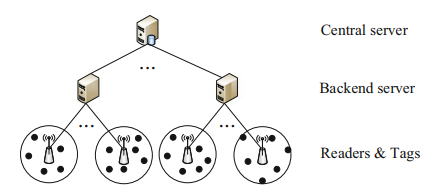
\includegraphics[width=\textwidth]{leightweight} 
\caption{\label{fig:lightweight} The system model of Lightweight Anonymous RFID Authentication \cite[p.40]{chen}} 
\end{figure}

Concerning the communication between readers and tags, Chen et al. describe a 'Request-Response mode Communication' \cite[p.40 ff.]{chen}. Firstly, the reader initiates the communication with the tag by sending a request to it. Secondly, after receiving the request, the tag makes an appropriate transmission as response. There can be distinguished two types of transmissions: Invariant and variant transmissions. The first type (invariant transmissions) can contain content that is 'invariant' between the tag and the reader. In contrast to that, variant transmissions can contain content that may vary for different tags or the same tag at different times, e.g. the exchanged data for anonymous authentication.  

\subsubsection{Identifying state-free networked tags}

Before explaining the mechanism of identifying state-free networked tags, the two terms 'state-free' and 'stateful' networked tags should be made clear. If a networked tag is called stateful, it maintains its networks state which includes information about its neighbors in the network, routing tables as well as update information. In contrast to that, state-free tags serve the purpose of energy conservation and do not maintain any network state prior to their operations which differs them from traditional networks. 
Given the two definitions, there comes up the challenge of identifying state-free networked tags. Chen et al. refer to that challenge and explain a method for identifying networked tags \cite[p.67 ff.]{chen} which will be discussed in the following. 
First of all, all tags in a network are connected to each other through a peer communication (to the nearby tags). Especially the emerging number of networked tags represents a significant enhancement to today's RFID technology. The problem of readers which cannot cover all tags due to cost or physical limitations can be solved by using networked tags. Moreover, the possibility of peer communication enables a multihop network to be formed among the tags. The transmission range of inter-tag communications is usually short and amounts to about 1-10 m whereas the transmission range of a reader is much larger. 
Nevertheless, the peer communication realizes a direct two-way communication between the current node and the neighboring node. Concerning the energy input, the energy can be powered through the reader's radio waves but the internal energy should be carried sufficiently for long-term operations (must be made energy-efficient).
After establishing a peer-to-peer communication, the reader collects the IDs from all networked tags that are in its read range. Using multiple hops and intermediate tags relaying the IDs of those tags which are not in the immediate coverage area of the reader, state-free tags can be identified. 

\subsection{RFID and Mobile Computing}

Concerning the development of mobile applications in context of the RFID technology, the following paragraph discusses fundamental definitions of mobile computing as well as general architecture patterns, like e.g. \ac{SOA}. 
To start with, Hanhart declares in his book \cite[p.9 ff.]{mobile} the term 'mobile computing' as following: '[...] all processes, activities, applications in a company which are proceed by mobile technologies. The company's staff gets access to data and applications (independently from location and time). The focus is set on man-machine-communication [...]' \cite[p.9 ff.]{mobile}. 
When it comes to mobile applications which are connected to RFID systems, Hanhart mentions the term of 'Smart things' or 'Embedded systems' which include physical objects, extended by the RFID sensor technology and which are networked to each other. To achieve some understanding among all readers, Hanhart depicts three types of wireless communications technology \cite[p.12-13]{mobile}. Firstly, there exist mobile communications which consist of a service provider and several mobile devices. The service provider transmits the speech and data from and to mobile devices through a wireless network. 
Secondly, Hanhart notices \ac{WLAN} which enables accessing to a company's network. To give an example, there exist many WLAN hotspots in hotels and airports, which can be accessed simply. Thirdly, there exist 'wireless personal networks' which connect terminal devices with peripheral devices within small ranges. For instance, Bluetooth or \ac{IrDA} are used to transfer data over small distances. Not only Bluetooth and infrared light are used to transfer data, but also ZigBees and \ac{NFC} is used in many cases \cite[p.12-13]{mobile}. Hanhart describes NFC as a newer technology which consists of an active and passive unit. Actually, NFC is only used for connections of a few centimeters, e.g. in consumer electronics. The active unit can be kept in the mobile because it is very small and the data rate amounts to at least 424 kbit/s.
 
\subsubsection{Basis functions of mobile computing and RFID}

When it comes to the use of mobile applications and RFID, one can distinguish between five general scenarios \cite[p.13 ff.]{mobile}. First of all, since RFID enables wireless connection and detection of several items in our environment, it can be used to access mobile applications through the RFID signal. For example, staff can use mobile devices to access (via RFID) business applications and to implement transactions. Secondly, as already mentioned in further sections above, RFID has the main purpose of identifying objects. In combination with mobile devices, there can be established applications which can both identify users and objects. As a third scenario, mobile RFID applications the capture of statal and environmental data. By using sensors, the continuous capture of data is possible. Moreover, smart objects and mobile devices can transform the information directly into actions or convey the data to a central system (or database). As a fourth scenario for using RFID in the context of mobile computing, Hanhart \cite[p.13 ff.]{mobile} remarks the possibility to locate precisely objects and users. Besides, the detected positions can be used to display contextual information or to direct to procedures in backend systems. Last but not least, the purpose of sending notifications in time, can improve and prevent several emergency situations (e.g. in a hospital). Since objects can send notifications e.g. when reaching a certain state, users get information everytime and everywhere.  

\subsubsection{Constraints of mobile applications and RFID}

Developing mobile applications with the RFID technology not only brings advantages, but also challenges when facing for example the user's needs and requirements. Hanhart indicates some 'constraints' of mobile applications and RFID \cite[p.16 ff.]{mobile} which will be depicted in the following. Firstly, the user interface should be considered. In case of healthcare applications which can be used by nurses, staff and physicians there should exist various user roles and rights. Thus, each user needs his specific interface and only a few (or one single) users are able to see all information of a patient. As a further matter, the mobile application should meet the requirements of connecting quality and service quality. This indicates the exact adaption of a service, specified in the requirements specification document. By the same, the challenge of computing capacity in the developer team should be attended. Furthermore, both principal and agent should be aware of the needed development time to realize all required features (which depends on the size and skill level of the developers). In addition, the technical resources, like e.g. memory capacity and energy supply represent another challenging factor. To deal with the last mentioned challenges, it should be favourable to have some sponsors which can support the project.

\subsubsection{Service-oriented architectures}

To cope with the constraints and challenges during the development of a mobile RFID application, Hanhart describes \ac{SOA} \cite[p.31 ff.]{mobile}. SOA is a multilayered, distributed information system architecture which encapsulates parts of an application into business-like services, considering design principles to enable a simplified process integration \cite[p.32]{mobile}. A service can be seen as an abstract software element or interface which provides standardized access to application functions of other applications through a network \cite[p.32]{mobile}. There exist four general design principles with respect to the development of SOA applications. The first design principle is called 'Orientation of Interfaces' which means that the service interfaces abstract implementation from the user's view. What is more, each service has a stable interface which is technically and functionally defined by its metadata. The second design principle of SOA is 'Interoperability' which can be assured by implementing technical and functional standards. This enables the interoperability of a services and its usage in different contexts. The third design principle is called 'Autonomy and Modularity' which signifies that SOA restructures the applications architecture into autonomous subsystems (domains and services). The aim is to increase cohesion in one system and to minimize the linkage between its subsystems. The fourth design principle of SOA is 'Orientation of needs'. This implies that all services should be oriented towards business objects and process activities in order to provide an approximately granular, functional definable output. 

\paragraph{Domain Architecture}

The Domain Architecture is a conceptional foundation of SOA. It reveals duplicates in an existing application architecture. Moreover, it is a fundamental decision foundation for service characteristics. Last but not least, it gives a list of possible service candidates which support systematic integration, development and usage of services.

\subsubsection{Service-oriented proposal of architecture}

In the previous section, the general characteristics of SOA have been discussed. But in which context SOA applications are regularily used? And how is SOA realized? To give answers to these questions, in the following the purpose and integration procedure of SOA applications will be explained. 
First of all, the conditions and prerequisites for an economic realization of diverse solutions based on mobile computing and RFID are simple and flexible integration into existing system architectures \cite[p.133 ff.]{mobile}. The classical integration of mobile terminal devices involves different middleware components and functions which can have different varieties of architecture (with advantages and disadvantages). Modern application systems are multilayered, for example 3-tier/n-tier-architectures. The three tiers include the client (implemented software-components), middleware (necessary components to connect client and backend) and backend (business data and functions) tier. The term 'mobile middleware' refers to the extension of the classical client-server architecture with the aim of improved scalability and administration.
Not only a mobile middleware is needed for an appropriate integration into SOA, but also a RFID middleware is needed. The following paragraph will mention some functional requirements to this specific middleware. First of all, transformation functions are needed to convert RFID raw data into useful business process data. This includes filtering of errors as well as harmonizing the data formats of different device manufacturers. Secondly, there are configuration functions needed for monitoring and controlling the RFID infrastructure. As follows, a configuration function is able to identify readers, manage configuration data, monitor device functionality and ensure security.  

\paragraph{Classic Integration Mechanism}

As a third type of integration, concerning mobile computing and RFID, the integration of embedded devices should be considered. Basically, there are three different tiers: Field tier, Automation tier and Management tier. The first tier, Field tier includes the physical connection of sensors, actuators and control units. The second tier, Automation tier, consists of control units which undertake automatic monitoring and processing functions, like for instance the control of temperature. The communication units connect the control units, programming units and the management tier. The third tier, called Management tier, subsists of monitor and control systems and visualizes them to the operator. Additionally, the Management tier delivers software responsive over proprietary interfaces and can be seen as data handling unit. 
To conclude, the Automation tier can be seen as the communication unit and middleware between Field tier and Management tier. Further, Automation and Management tier can connect to third-party-applications via data interface units.
 
\paragraph{Modern Integration Mechanism}

The last paragraph dealed with integration mechanisms on the real old way. Recently, there are newer technologies and possibilities to realize an integration, such as web services and the emerging communication protocol \ac{SOAP}. In context of web technologies and services, there comes up the term \ac{ESB} \cite[p.141 ff.]{mobile} which provides a standardized interface and communication layer. An ESB is a consistent integration architecture which defines standards as well as central services and provides them for software development, publication and usage. Regarding the integration of mobile applications, the ESB \cite[p.143]{mobile}, there are differentiated two types of integration scenarios: a) the mobile client calls directly the provided services from application domains or b) the client keeps communicating with the services via its mobile middleware. If the client wants to call a service directly, he has to implement its \ac{API}. Besides, for service call or invocation, the standardized interface technology has to be used.
In the matter of integration of RFID systems and embedded devices, the middleware of RFID systems uses the provided services of the application domains, provided by the ESB. In addition to that, mobile applications can be integrated both online and offline \cite[p.146 ff.]{mobile}. Hanhart is using the term 'online' in context of saying that the mobile device runs the user interface. This indicates that the mobile middleware prepares contents of application (for prompt). After that, the application accesses the backend or invoked app through a service which uses the application's functionality via services. In contrast to that, Hanhart uses the expression 'offline' in order to say that the application is running on the client. Here, the mobile application acts as an invoked application and synchronizes its data through the mobile middleware with the backend. The central management of process states (on the client) and synchronization with services are realized through the middleware directly.

\paragraph{Capabilities of SOA, mobile applications and RFID}

To explain the capabilities of the above discussed technologies and architecture, Hanhart brings up 'Reuse', 'Isolation of Domains' and 'Easy implementation'. Reuse is generated by consistent functionalities of interfaces. Isolation of domains is produced by separation of concerns and core data concepts. Easy implementation refers to cross-domain workflows or taskflows. Concerning possible usage scenarios, Hanhart mentions some examples \cite[p.207 ff.]{mobile}, like event-driven process management which includes the automatic capture of events. Or, if it comes to the control of several processes and activities in a company, these activities can be executed by using mobile phones or tablets. Additionally, they will record the encountered states.
Concerning the 'ecosystem' and exchanges in it, Hanhart talks about some upcoming challenges \cite[p.212 ff.]{mobile}, like the realization of mobile solutions. It is important to consider the high costs of hardware and software. In addition to that, the complexity of integration of solutions and backend systems has to be assumed very well. Lastly, there should be staff who configures and operates the mobile devices.  

\paragraph{Examples of SOA applications}

Hanhart mentions several use cases of mobile applications and RFID. In order to depict two of his examples, the following paragraph will explain firstly the case study: 'Fraport AG' \cite[p.39 ff.]{mobile} and secondly a \ac{WfMS} \cite[p.204 ff.]{mobile}. To start with, Fraport AG is a company which is simulataneously owner and operator of Frankfurt airport. By including the RFID technology and mobile devices, several solutions have been realized in processes for mobile support of staff and in use of real-time data. The scope contained the maintainance of fire dampers and mobile support of loadmasters during loading respectively unloading and mobile capture of booking of goods input and goods issue in stock. 
The second example Hanhart notices, is a WfMS \cite[p.204 ff.]{mobile} which is able to control processes, e.g. in companies. To realize a WfMS, the workflow client needs to be installed on the mobile device. Following, RFID systems and embedded devices are able to report events to WfMS and can trigger or control processes on the workflow integration layer.
     
To give an outlook of the possible extensions of mobile applications and RFID, Hanhart explains some fundamental concepts \cite[p.208 ff.]{mobile}. The first concept is called 'Emotion-Silent Process' and is based on sensors, actuators, artificial intelligence which includes the learning from given data and derive several activities. In the given usage scenario (which refers to a hospital or retirement home), sensors firstly detect the movement of a elder person. After the detection step, the sensor's information are connected to further data (e.g. time) with the help of pattern detection algorithms. Finally, the aim of the 'Emotion-Silent Process' is to detect and prevent emergency situations by sending an alarm to responsible persons (like physicians or nurses). Furthermore, the process is called 'Emotion-Silent Process' because of the 'silent' protection of people which should obtain the independance of these people.
A second usage scenario which is noticed, is called 'Velocity-Outtasking and Application Outsourcing'. Based on the spread of web services in cross-company cooperations either external access to single tasks and functions ('outsourcing') or to whole applications ('application outsourcing') can be accelerated. 
The term 'Outtalking' is used to talk about web services of external providers which can be incorporated to the own service repository and are centrally available for further usage. In contrast to that, 'Application Outsourcing' refers to externally obtained applications (from \ac{ASP}) which can be integrated through the company-internal ESB into the system landscape.

\section{Analysis of RFID applications and their use}

Often, there not only exists one ideal solution for implementing RFID applications, but multiple applications. In order to decide whether the proposed solution is the appropriate one, the \ac{SWOT} method has been established \cite[p.47 ff.]{fokus}. SWOT is the acronym for strengths-weaknesses-opportunities-threats and can be seen as the epitome of a popular instrument for self-analysis of decision makers. The analysis itself can be divided into two comprising steps: In order to achieve the objective with the given system, its strengths and weaknesses (with an internal origin) are identified in the first step. After that, the system's environment is analyzed by ascertaining external opportunities and threats. 
To give an example of the SWOT analysis, Tamm and Tribowski \cite[p.47 ff.]{fokus} consider two perspectives on RFID applications: The 'Enterprise Perspective' as well as the 'Political Perspective' which will be described in the following. 
From the enterprise's point of view, the strengths of RFID systems are the optimization of operational processes and the reduction of costs. Further, many enterprises improve their transparency because of the raised quality of data (improved decision making). In contrast to that, there exist weaknesses of RFID applications from the view of enterprises, e.g. the challenge of integrating them into the IT, the physical as well as the organizational integration of processes. When it comes to the environmental analysis of enterprises, there occur some opportunities, like for example new business models which are based on RFID. Or, for instance there will arise innovative business partners which cause a general willingness to cooperate with them. On the opposite, there also might occur some threats in the context of RFID applications in enterprises. To give an example, there might appear an asymmetrical cost-benefit in the value chain. Moreover, any application standards are missing to establish a cross-company infrastructure \cite[p.47 ff.]{fokus}.
From the political perspective, the strengths of RFID applications are receptive RFID users, effective manufacturers of the technology, exploratory infrastructure and strategic projects. In contrast to that, the weaknesses of the mentioned systems could be the risk of investment at \ac{SME}, an inadequate alignment of the technology in Europe and missing application standards. As external opportunities can be seen the high potential to gains in efficiency, the emerging new employments, the market share for european technology manufacturers and the resulting data privacy technologies. On the other hand,  Tamm and Tribowski \cite[p.47 ff.]{fokus} mention political threats which might exist in the german point of view. For instance, there might occur competitions in technology development with the USA and Asia, rising discounters beyond Europe, missing global interoperability as well as a missing consensus of sociopolitical problems. 

According to Tamm and Tribowski \cite[p.95 ff.]{fokus}, the highest potential of the RFID applications is the cross-company deployment of RFID because of the raised visibility in a cross-company solution. Generally, the benefit of network technologies depends on the deployment of the application in the network as well as on the number of partners which are integrated into the application. Nevertheless, cross-company RFID solutions enable cost reduce due to the distribution of costs to multiple stakeholders and because of the multipurpose of their transponder.

\subsection{Process Model}

When establishing a RFID system in a company or building a cross-company infrastructure, in practice, process models are used to roll out. Process models divide a process into definite phases \cite[p.59 ff.]{fokus} which can be named as the following: 1) prephase, 2) analysis phase, 3) draft phase, 4) implementation phase and 5) adoption phase. In the succeeding paragraph, each phase will be depicted briefly.
Firstly, the prephase includes the definition of determine aims, the project team, requirements to the application, funding models and approach. After that, in the second phase (analysis phase) information about all stakeholders is collected. Afterwards, all used IT systems are analyzed in order to integrate the RFID technology correctly into existing applications. Besides, the technical infrastructure is analyzed to find out the technical characteristics of RFID. In addition to that, the functional requirements are defined.
In the third phase, the draft phase, the target process is the documentation of the functional specification document which is based on the specification book. Next, during the implementation phase, the software is developed and tested, hardware installation, configuration, tests are performed. Every action as well as every result is documented and later used as training material. All in all, this phase aims to implement an operational solution which can be adopted to the existing systems. 
Before the last phase, qualification measures for all stakeholders are performed in order to check the appropriateness of the application to the specified requirements of phase three.
In the last phase, the adoption phase, the developed application is adopted and released. With the adoption, the maintainance phase of the application starts.
To conclude this recommended process model, one should consider that it is only a 'model' described by Tamm and Tribowski \cite[p.59 ff.]{fokus}and project-specific variables like e.g. number of team members or ressources can influence each of the stated phases.